\documentclass[12pt]{article}
\usepackage{fullpage}
\usepackage{amsmath,amssymb,amsthm}
\usepackage{xcolor,soul}
\usepackage{mparhack}
\usepackage[utf8]{inputenc}
\usepackage{dsfont}
\usepackage{graphicx}
\usepackage{tikz}
\usepackage{float}
\usepackage{subfig}
\usepackage{hyperref}
\usepackage{stmaryrd}
\usepackage{esint}
\usepackage{braket}
\usepackage{verbatim}
\usepackage{thmtools}
\usepackage{relsize}
\SetSymbolFont{stmry}{bold}{U}{stmry}{m}{n}
\usepackage{bm}

\newcommand{\cmark}{\ding{51}}%
\newcommand{\xmark}{\ding{55}}
\newcommand{\subfigureautorefname}{\figureautorefname}
\declaretheorem[numberwithin=section,name=Theorem,refname={Theorem,Theorems}, Refname={Theorem,Theorems}]{theorem}
\declaretheorem[numberwithin=section,name=Lemma, refname={Lemma,Lemmas},Refname={Lemma,Lemmas}]{lemma}
\declaretheorem[numberwithin=section,name=Corollary, refname={Corollary,Corollaries},Refname={Corollary,Corollaries}]{corollary}
\declaretheorem[style=remark]{Sketch of proof}
\declaretheorem[numbered=no, name=Remark]{remark}
\newcommand{\annotation}[1]{\marginpar{\small\color{red}#1}}

\title{Implicit Integration for Density of States}
\date{}
\author{Ewen Lallinec$^1$}

\begin{document}
\maketitle
\footnotetext[1]{Université Paris-Saclay, CNRS, Laboratoire de mathématiques d’Orsay, 91405, Orsay, France}

\section{Quantum formalism}
\subsection{Periodic infinite crystal}
Let $\mathcal{R}$ be a discrete periodic lattice of $\mathbb{R}^d$ (for $d \in \left\{1,\dots, 3\right\}$)
\begin{equation}
	\mathcal{R} = \left\{\sum_{i=1}^d n_i \mathbf{a}_i= A\mathbf{n} , \, n_i \in \mathbb{Z} \right\},
\end{equation}
where $A=(\mathbf{a}_1\dots\mathbf{a}_d) \in \mathbb{R}^{d\times d}$ is non-degenerate.\\
We denote $\Gamma$ its unit cell (the Wigner-Seitz cell centered around $\mathbf{0}$).
\begin{equation}
	\Gamma = \left\{\mathbf{r} \in  \mathbb{R}^d, \lVert \mathbf{r} \rVert_ 2\leq\lVert \mathbf{r}- \mathbf{R}\rVert_2, \ \forall \ \mathbf{R} \in  \mathcal{R}\backslash\{\mathbf{0}\}\right\}.
\end{equation}
Now let's define $\mathcal{R}^*$ the reciprocal lattice associated to $\mathcal{R}$

\begin{equation}
	\mathcal{R}^* = \left\{\sum_{i=1}^d n_i \mathbf{b}_i=B\mathbf{n}, \, n_i \in \mathbb{Z}\right\},
\end{equation}
where $A^\intercal  B= 2\pi I$.

We now define the Brillouin zone $\mathcal{B}$ as the Wigner-Seitz cell centered around $\mathbf{0}$ in the reciprocal lattice
\begin{equation}
	\mathcal{B} = \left\{\mathbf{k} \in  \mathbb{R}^d, \lVert \mathbf{k} \rVert_ 2\leq\lVert \mathbf{k}- \mathbf{G}\rVert_2, \ \forall \ \mathbf{G} \in  \mathcal{R}^*\backslash\{\mathbf{0}\}\right\}
\end{equation}
\subsection{Supercell method}
For $L \in \mathbb{N}$, we define the supercell as
\begin{equation}
	\Gamma_L=L\Gamma,
\end{equation}
corresponding to $L$ replication of the unit cell along each lattice direction.
Now we naturally define the truncated lattice $\mathcal{R}_L$ as
\begin{equation}
	\mathcal{R}_L = \mathcal{R}\cap \Gamma_L.
\end{equation}
This structure induces a discretization of the Brillouin zone by exploiting the duality between $\mathcal{R}$ and $\mathcal{R}^*$. We define this discretized Brillouin zone $\mathcal{B}_L$ as
\begin{equation}
	\mathcal{B}_L = \left\{ \sum_{i=1}^d \frac{n_i}{L} \mathbf{b}_i \;\middle|\; n_i \in \left\{-\left\lfloor\frac{L}{2}\right\rfloor, \ldots, \left\lfloor\frac{L}{2} - 1\right\rfloor \right\} \right\}.
\end{equation}

\subsection{Hamiltonian and bands}
Now we consider a Bloch Hamiltonian defined as the truncated Bloch transform of given real space Hamiltonians $H_\mathbf{R}$
\begin{equation}
	H:\left\{
	\begin{matrix}\mathcal{B} \rightarrow \mathbb{C}^{M \times M} \\
		\displaystyle{\mathbf{k} \mapsto \sum_{\mathbf{R} \in \mathcal{R}_L} \mathrm{e}^{i \mathbf{k} \cdot \mathbf{R}} H_{\mathbf{R}}}\end{matrix}\right. .
\end{equation}
This Hamiltonian is $\mathcal{R}^*$-periodic and is a Hermitian matrix which verifies the time-independent Schrödinger equation at each $\mathbf{k}$ of $\mathcal{B}$

\begin{equation}
	H(\mathbf{k}) \psi_{m}(\mathbf{k}) = \varepsilon_{m} (\mathbf{k}) \psi_{m}(\mathbf{k}),
\end{equation}
where $\psi_m$ and $\varepsilon_m$ respectively are the m-th eigenvectors and eigenvalues of $H$.

\subsection{Density of states}
The Density of States (DOS) is defined as
\begin{equation}
	D(E) = \frac{1}{|\mathcal{B}|}\sum_{m=1}^M\int_{\mathcal{B}}\delta(E-\varepsilon_m(\mathbf{k}))\mathrm{d}\mathbf{k}
\end{equation}
A change of variable (co-area formula) gives another expression
\begin{equation}\label{eq:dosgrad}
	D(E)=\frac{1}{|\mathcal{B}|}\sum_{m=1}^M\int_{S_m(E)} \frac{1}{|\nabla\varepsilon_{m}(\mathbf{k})|}\mathrm{d}\mathcal{H}^{d-1}(\mathbf{k})
\end{equation}
where $\mathrm{d}\mathcal{H}^{d-1}(\mathbf{k})$ is the Haussdorff measure of dimension $d-1$ and the $S_m(E)$ are isosurfaces of the m-th eigenvalue
\begin{equation}
	S_m(E) = \left\{\mathbf{k} \in \mathcal{B}, \varepsilon_{m}(\mathbf{k})=E \right\}.
\end{equation}
From~\autoref{eq:dosgrad}, we can define the DOS as a sum of integrals over implicitly defined surfaces, the $S_m(E)$. Therefore the method of implicit integration~\cite{saye_high-order_2015} can be meaningful if we manage to bound efficiently the different eigenvalues on intervals.


\section{High-Order Quadrature Methods for Implicitly Defined Surfaces and Volumes in Hyperrectangles}
The idea of this algorithm is to compute integrals of sufficiently smooth function $f$ on implicitly defined surfaces (with $U\subset \mathbb{R}^d$ a given hyperrectangle).
\begin{equation}
	\int_{\Gamma\cap D} f
\end{equation}
where $\Gamma$ is a surface defined implicitly $\Gamma = \{x \in \mathbb{R}^d \, | \, \phi(x)=0 \}$.
\begin{comment}
\begin{equation}
	\Gamma=\{x:\phi(x)=0\} \ \mathrm{and}\ \Omega=\{x : \phi(x)<0\}
\end{equation}

The first one is a volume integral, whereas the second one is a surface integral (respectively on spaces of dimension $d$ and $d-1$).

\textbf{Applications}
Globally level-set methods
\begin{itemize}
	\item Propagation of interfaces in computational physics
	\item Embedded boundary methods to solve PDEs on curved domains
	\item Jump conditions and singular source terms
\end{itemize}

\subsection{Usual approachs}
\begin{itemize}
	\item[-] (Numerically discrete) Delta or Heaviside functions
		\begin{align}
			\int_\Omega f & = \int_V f \delta(\phi) \Big|\nabla\phi\Big|\approx h^d \sum_i f(x_i)\delta_h(\phi(x_i))\Big|\nabla\phi(x_i)\Big|\label{eq:omega} \\
			\int_\Gamma g & = \int_V g H(-\phi) \approx h^d \sum_i g(x_i) H_h(-\phi(x_i))\label{eq:gamma}
		\end{align}
		\begin{itemize}
			\item[$\bullet$] Pros: simple to understand, to implement.
			\item[$\bullet$] Cons: Works only for smooth surfaces, surfaces with boundaries. Highly dependent on the discretization and the approximation of $\delta$/$H$ (sometimes no convergence achieved).
		\end{itemize}
	\item[-] Divergence theorem to reduce recursively the problem to lower dimension integrals
		\begin{equation}
			\int_{\Omega\cap U}f= \int_{\Omega\cap U} \mathrm{div}(\mathbf{u}) = \int_{\partial(\Omega\cap U)}\mathbf{u}\cdot\mathbf{n}= \int_{\Gamma\cap U}\mathbf{u}\cdot\mathbf{n} +\int_{\Omega\cap \partial U}\mathbf{u}\cdot\mathbf{n}
		\end{equation}
		If we can choose $\tilde{\mathbf{u}}$ such that $\mathrm{div}(\tilde{\mathbf{u}})=0$ on $U$ and $\tilde{\mathbf{u}}\cdot\mathbf{n}=g$ on $\Gamma$ then
		\begin{equation}
			\int_{\Gamma\cap U}g=-\int_{\Omega\cap \partial U}\tilde{\mathbf{u}}\cdot\mathbf{n}
		\end{equation}
		\begin{itemize}
			\item[$\bullet$] Pros: Reduces the dimension of the problem, recursive and easy to understand for most cases.
			\item[$\bullet$] Cons: Doesn't work if $\Gamma\cap\partial U=\emptyset$ which depicts the facts that we can't always find a divergence-free $\tilde{\mathbf{u}}$. Moreover it needs to suppose that $g$ is smooth enough to be smoothly extended outside of $\Gamma$ and that $\nabla \phi$ was smooth throughout $U$.
		\end{itemize}
	\item[-] Explicit reconstruction of the surface (the most computationally expensive method)
		\begin{itemize}
			\item[$\bullet$] Pros
			\item[$\bullet$] Cons
		\end{itemize}
\end{itemize}
\end{comment}
\subsection{Quadrature on implicitly defined domains via dimension reduction}
The idea is to convert $\Gamma$ into the graph of an implicitly defined height function.
To do so we define an $d$-dimensional hyperrectangle $U$
\begin{equation}
	U=(x_1^L,x_1^U)\times\dots\times(x_d^L,x_d^U)
\end{equation}
and we denote by $(e_i)_{1\leq i\leq d}$ the canonical basis of $\mathbb{R}^d$.\\
For a sufficiently small $U$ and a smooth enough $\phi$ (at least $\mathcal{C}^1$), we have $|\partial_{x_i}\phi|$ which is bounded away from zero. Therefore we can apply the implicit function theorem to describe locally $\Gamma\cap U$ with a height function such that  $x_i=h(x_1,\dots,x_{i-1},x_{i+1},\dots,x_d)$ on $\left[ x_i^L,x_i^U \right]$.
\begin{equation}
	\phi(x_1,\dots,x_{i-1},h(x_1,\dots,x_{i-1},x_{i+1},\dots,x_d),x_{i+1},\dots,x_d)=0\label{eq:height}
\end{equation}
This is illustrated in~\autoref{fig:delimitation}.
\begin{figure}[H]
	\centering
	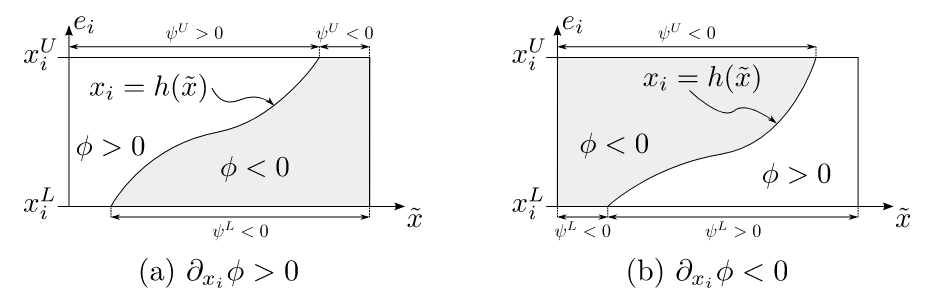
\includegraphics[scale=0.45]{Images/Hyperrectangle.png}
	\caption{Cases for the definition of $V_1$ and $V_2$ (image from~\cite{saye_high-order_2015})}
	\label{fig:delimitation}
\end{figure}
We define two functions $\psi^L$ and $\psi^U$ of $\tilde{x} = (x_1,\dots,x_{i-1},x_{i+1},\dots,x_d)$ which are the restrictions of $\phi$ to the lower and upper faces.
\begin{align}
	\psi^L(\tilde{x}) & = \phi(\tilde{x} + x_i^L e_i) \\
	\psi^U(\tilde{x}) & =\phi(\tilde{x} + x_i^U e_i)
\end{align}
This allows to define 2 $(d-1)$-dimensional volumes $V_1$ and $V_2$
\begin{align}
	V_1 & =\left\{
	\begin{matrix}
		\{\tilde{x}:\psi^L(\tilde{x})<0 \} & \mathrm{if} \ \partial_{x_i}\phi>0 \ \mathrm{in} \ U \\
		\{\tilde{x}:\psi^L(\tilde{x})>0 \} & \mathrm{if} \ \partial_{x_i}\phi<0 \ \mathrm{in} \ U
	\end{matrix}
	\right.        \\
	V_2 & =\left\{
	\begin{matrix}
		\{\tilde{x}:\psi^U(\tilde{x})>0 \} & \mathrm{if} \ \partial_{x_i}\phi>0 \ \mathrm{in} \ U \\
		\{\tilde{x}:\psi^U(\tilde{x})<0 \} & \mathrm{if} \ \partial_{x_i}\phi<0 \ \mathrm{in} \ U
	\end{matrix}
	\right.
\end{align}
From~\eqref{eq:height} we have $\mathrm{d}S = \sqrt{1+|\nabla_{\tilde{x}} h(\tilde{x})|^2}\mathrm{d}\tilde{x}$.
Moreover by derivating~\eqref{eq:height},
\begin{equation}
	\forall j\neq i, \partial_{x_j} h(\tilde{x}) = -\frac{\partial_j\phi}{\partial_i\phi }\biggr\rvert_{x=\tilde{x}+h(\tilde{x})e_i}
\end{equation}
Thus
\begin{equation}
	\sqrt{1+|\nabla_{\tilde{x}} h(\tilde{x})|^2} = \frac{|\nabla \phi|}{\left|\partial_i\phi\right|}\biggr\rvert_{x=\tilde{x}+h(\tilde{x})e_i}
\end{equation}
Using this equality yields
\begin{equation}
	\int_{\Gamma\cap U}g\mathrm{d}S=\int_{V_1\cap V_2}g \frac{|\nabla \phi|}{\left|\partial_i\phi\right|}\biggr\rvert_{x=\tilde{x}+h(\tilde{x})e_i}\mathrm{d}\tilde{x}
\end{equation}

Therefore this algorithm convergence depends on the correct localization of the isosurface $\Gamma$, and this localization itself intrinsically depends on the quality of the bounds on $\phi$ and its partial derivatives.

\subsection{Application to eh computation of the Density of States}
Now we want to apply this algorithm to the Density of States (DOS).
We remind that
\begin{equation}\label{eq:dosgrad}
	D(E)=\frac{1}{|\mathcal{B}|}\sum_{m=1}^M\int_{S_m(E)} \frac{1}{|\nabla\varepsilon_{m}(\mathbf{k})|}\mathrm{d}\mathcal{H}^{d-1}(\mathbf{k}),
\end{equation}
which can be computed using the above-presented algorithm applied at each eigenvalue minus the desired energy level. We write

\begin{equation}
	\phi_{m,E} = \varepsilon_m-E
\end{equation}

In our case we will focus on the case of boxes centered around points $\mathbf{k}_0$, we will denote the box $\bm{\delta k}$ and the box centered around $\mathbf{k}_0$ as $D=\bm{\delta k}+\mathbf{k}_0$

\section{Time-independent perturbation theory}
We want to find approximations of the eigenvalues $\varepsilon_m$ and eigenstates $\psi_m$ of a Hamiltonian $H$. To do so we express $H$ as a small perturbation of a reference Hamiltonian $H_0$ by a small parameter $\lambda$. Then using a serie expansion in $\lambda$ we can find approximations of $H$ eigenvalues/eigenstates depending on $H_0$ eigenvalues $\varepsilon_{m,0}$ and eigenstates $\psi_{m,0}$.\\
Let $H$, $H_0$ and $\delta H$ be three Hamiltonian of $\mathbb{C}^{M\times M}$ such that

\begin{equation}
	H(\lambda) = H_0+\lambda \delta H
\end{equation}
where $\lambda $ is a small positive parameter.\\
We define for $m\in \llbracket 1, M \rrbracket$
\begin{equation}
	H\psi_m=\varepsilon_m\psi_m
\end{equation}
and

\begin{equation}
	H_0\psi_{m,0}=\varepsilon_{m,0}\psi_{m,0}
\end{equation}
Now considering a non-degenerate eigenvalues $\varepsilon_m(\lambda)$. We expand it in series as

\begin{equation}
	\varepsilon_m(\lambda) = \sum_{i=0}^{+\infty}\lambda^i\varepsilon_m^{(i)}
\end{equation}
Using the normalization of Hamiltonian eigenstates ($\lVert\psi\rVert_2=1$) and identifying each term in the development we have at second-order that

\begin{equation}
	\varepsilon_m(\lambda) = \varepsilon_{m,0} + \lambda \braket{\psi_{m,0}| W| \psi_{m,0}} + \lambda^2 \sum_{n\neq m} \frac{\braket{\psi_{n,0}| W| \psi_{m,0}}^2}{\varepsilon_{m,0}-\varepsilon_{n,0}} +\mathcal{O}(\lambda^3)
\end{equation}
Now considering a sufficiently smooth (at least continously differentiable) Hamiltonian $H_{\mathbf{k}}$ at point $\mathbf{k}$ of the Brillouin zone. We want its Taylor expansion around point $\mathbf{k}_0$, we write  $\delta_\mathbf{k} = (\delta_{k_i})_{i \in \{1,\dots,d\}} = (k_i-k_{0,i})_{i \in \{1,\dots,d\}}$. Here the perturbation theory yields

\begin{equation}
	\varepsilon_{m}(\mathbf{k}) = \varepsilon_{m}(\mathbf{k}_0) + \mathlarger{\sum_{i \in \{1,\dots,d \}}}\frac{\partial\varepsilon_{m}(\mathbf{k}_0)}{\partial k_i}\delta_{k_i}+\frac{1}{2}\mathlarger{\sum_{i,j \in \{1,\dots,d \}}} \frac{\partial^2\varepsilon_{m}(\mathbf{k}_0)}{\partial k_i\partial k_j}\delta_{k_i} \delta_{k_j}+\mathcal{O}(\lVert k\rVert^3) \label{eq:perteigen}
\end{equation}
where
\begin{equation}
	\frac{\partial\varepsilon_{m}}{\partial k_i} = \braket{\psi_{m}| \partial_{i} H| \psi_{m}}
\end{equation}
and
\begin{equation}
	\frac{\partial^2\varepsilon_{m}}{\partial k_i\partial k_j}=\braket{\psi_{m}| \partial_{i}\partial_{j}H| \psi_{m}}+
	2\sum_{n\neq m}\frac{\mathrm{Re}\left(\braket{\psi_{m}| \partial_{i}H| \psi_{n}}\braket{\psi_{n}| \partial_{j}H| \psi_{m}}\right)}{\varepsilon_{m}-\varepsilon_{n}}
\end{equation}
\subsection{Guaranteed theoretical bound}
Now from~\autoref{eq:perteigen} we can derive guaranteed bounds on the eigenvalues.\\
\textcolor{red}{Introduire les notations avant pour $H$, $\varepsilon_m$,$\psi_m$, $\delta \mathbf{k}$  et $D$}
\begin{lemma}{Weyl's Inequality for Bloch eigenvalues}\label{lemma:weyl}\\
	Let $\mathbf{k}_0 \in \mathcal{B}$ and $H: \mathcal{B} \rightarrow \mathbb{C}^{M \times M}$ an analytic Bloch Hamiltonian. Let $D=\bm{k_0}+\bm{\delta k}=\left\{\mathbf{k} \in \mathcal{B}, |k_i-k_{0,i}|\leq \delta k_i, \, i \in\{1,\cdots,d\} \right\}$ the hyperrectangle centered around $\mathbf{k}_0$.\\
	Then for all $m=1,\dots,M$, $ \mathbf{k} \in D$,
	\begin{equation}
		|\varepsilon_{m}(\mathbf{k}) - \varepsilon_{m}(\mathbf{k}_0)| \leq \sup_{\mathbf{q} \in D}\lVert H(\mathbf{q})-H(\mathbf{k}_0)\rVert_{\mathrm{op}}
	\end{equation}
	where $\lVert\cdot \rVert_{\mathrm{op}}$ denotes the operator norm defined as

	\begin{equation}
		\lVert H \rVert_{\mathrm{op}} = \sup_{\lVert \psi \rVert_2\, =1} \lVert H \psi \rVert_2 .
	\end{equation}

\end{lemma}

\begin{corollary}[First-order bound]

	In addition, if $\varepsilon_m$ is non-degenerate, then for all $ \mathbf{k} \in D$,

	\begin{equation}
		|\varepsilon_{m}(\mathbf{k}) - \varepsilon_{m}(\mathbf{k}_0)|
		\leq
		\sup_{\mathbf{k} \in D}\sum_{j=1}^d \lVert\partial_j H(\mathbf{k})\rVert_{\mathrm{op}} |\delta k_j|
		\leq
		\sup_{\mathbf{k} \in D}\sqrt {\sum_{j=1}^d\left\lVert\partial_j H(\mathbf{k})\right\rVert_{\mathrm{op}}^2}\lVert \delta \mathbf{k} \rVert_2
	\end{equation}
\end{corollary}
\begin{proof}
	Let $\mathbf{k} \in D$, we suppose that each eigenvalue is non-degenerate in $D$.\\
	Let $\gamma: t\mapsto (1-t)\mathbf{k}_0 +t\mathbf{k}$ a straight-line path between $\mathbf{k}$ and $\mathbf{k}_0$.
	We define $f:t \mapsto H(\gamma(t))$ which is analytic by composition.
	The chain rule yields
	\begin{equation}
		f'(t) = \sum_{j=1}^d \partial_j H(\gamma(t))(k_j - k_{0,j}).
	\end{equation}
	Hence
	\begin{equation}
		H(\mathbf{k})-H(\mathbf{k}_0) =f(1)-f(0)= \int_0^1 f'(t)\mathrm{d}t = \sum_{j=1}^d\int_0^1 \partial_j H(\gamma(t))(k_j - k_{0,j}).
	\end{equation}
	Taking the operator norm and applying the triangular inequality gives
	\begin{equation}
		\lVert H(\mathbf{k})-H(\mathbf{k}_0)\rVert_{\mathrm{op}} \leq \sum_{j=1}^d \int_0^1 \lVert\partial_jH(\gamma(t))\rVert_{\mathrm{op}}|k_j - k_{0,j}|\mathrm{d}t \leq  \sum_{j=1}^d  \lVert\partial_jH(\gamma(t))\rVert_{\mathrm{op}}|\delta k_j| .
	\end{equation}
	Now by combining that $\forall t \in [0,1], \gamma(t) \in D$ and the~\autoref{lemma:weyl}
	\begin{equation}
		|\varepsilon_{m}(\mathbf{k}) - \varepsilon_{m}(\mathbf{k}_0)|
		\leq
		\lVert H(\mathbf{k})-H(\mathbf{k}_0)\rVert_{\mathrm{op}}
		\leq
		\sup_{\mathbf{q} \in D}\sum_{j=1}^d \lVert\partial_j H(\mathbf{q})\rVert_{\mathrm{op}} |\delta k_j|.
	\end{equation}
	Finally, Cauchy-Schwarz inequality gives the second bound
	\begin{equation}
		|\varepsilon_{m}(\mathbf{k}) - \varepsilon_{m}(\mathbf{k}_0)|
		\leq
		\sup_{\mathbf{k} \in D}\sqrt {\sum_{j=1}^d\left\lVert\partial_j H(\mathbf{k})\right\rVert_{\mathrm{op}}^2}\lVert \delta \mathbf{k} \rVert_2
	\end{equation}
	This concludes the proof.
\end{proof}

\begin{corollary}[Second‐order bound]

	Under the same non-degeneracy hypothesis on $\varepsilon_m$, we have for all $ \mathbf{k} \in D$,
	\begin{equation}
		|\varepsilon_{m}(\mathbf{k}) - \varepsilon_{m}(\mathbf{k}_0) -\sum_{i=1}^d \delta k_i \frac{\partial \varepsilon_m}{\partial k_i}(\mathbf{k}_0)| \leq  \frac{1}{2}\lVert \delta \mathbf{k} \rVert_2^2 \sup_{\mathbf{k} \in D}\left( \lVert \nabla^2 H(\mathbf{k})\rVert_{\mathrm{op}}+ 2\frac{\lVert \nabla H(\mathbf{k})\rVert^2_{\mathrm{op}}}{\Delta_m}\right)
	\end{equation}
	where $\displaystyle{\Delta_m = \min_{\mathbf{k}_1, \mathbf{k}_2 \in D, n\neq m} |\varepsilon_m(k_1) -\varepsilon_n(k_2) |}$ is the gap between the $m$-th eigenvalue and the closest eigenvalue of a different band.

	\begin{proof}
		The idea is to use the second term of the Taylor expansion of our eigenvalue.
		Let $\mathbf{k} \in D$,

	\end{proof}
\end{corollary}

\subsection{Numerical bounds}
The theoretical bounds are valid, but we often don’t know the exact supremum of our eigenvalues on a given box. To ensure our algorithm performs reliably, we need numerical estimates. One approach is to use interval arithmetic. Although the bounds from interval arithmetic aren’t sharp, they are rigorous—especially since our Hamiltonians are represented as truncated Fourier series of known matrices. Our strategy, then, is to combine and compare several different eigenvalue bounds to find the most effective estimate.

\subsubsection{Interval Arithmetic}
We remind the  Taylor expansion for functions over an interval
\begin{equation}
	[f]([x]) = f(y)+\sum_{|\alpha|=1}^{k} \frac{D^\alpha f(y)}{\alpha!}([x]-y)^\alpha + \sum_{\alpha=|k+1|}\frac{[D^{|\alpha|}f]([x])}{(\alpha)!}([x]-y)^{\alpha}
\end{equation}
where $\alpha= (\alpha_1,\dots,\alpha_d)$ , $\displaystyle{\alpha! = \prod_{i=1}^d \alpha_i!}$, $\displaystyle{D^\alpha f=\frac{\partial^{\alpha}f}{\partial k_1^{\alpha_1}\dots \partial k_d^{\alpha_d}}}$ and $\displaystyle{([x]-y)^\alpha}= \prod_{i=1}^{d}([x]-y)^{\alpha_i}$.\\
In our case up to first and second order we have

\begin{equation}
	[\varepsilon_m]([\bm{\delta k}]+\bm{k}_0) = \varepsilon_m(\mathbf{k}_0)+ \sum_{i=1}^d[\partial_i\varepsilon_m]([\bm{\delta k}]+\mathbf{k}_0)[\delta k_i]
\end{equation}
\begin{equation}
	[\varepsilon_m]([\bm{\delta k}]+\bm{k}_0) = \varepsilon_m(\mathbf{k}_0)+ \sum_{i=1}^d\partial_i \varepsilon_m(\mathbf{k}_0)\cdot[\delta k_i]+ \sum_{i,j = 1}^d\frac{[\partial_i\partial_j\varepsilon_m]([\bm{\delta k}]+\bm{k}_0)}{2!}\cdot[\delta k_i][\delta k_j]
\end{equation}
\subsubsection{Sampling bounds}
The idea of sampling bounds is to get non-guaranteed bounds but which tends to the real bounds as the number of sampling points tends to infinity. The idea is to use the bounds obtained in~\autoref{lemma:weyl} and to obtain an estimation of the sup of the desired quantities to directly use our bounds.

\textcolor{red}{Cette partie là on fait pas du coup si j'ai bien compris}
\section{Bounds for degenerate eigenvalues}
For degenerate eigenvalues, the Hamiltonian regularity does not imply the regularity of its eigenvalues. Thus the classical perturbation theory is not fitted to bound the eigenvalues after the first-order.

Let $\mathbf{k}_0 \in \mathcal{B}$ such that $\varepsilon_{i}, \varepsilon_{j}$ are degenerate eigenvalues. Let $P$ be the projector on the eigenspace spanned by the corresponding eigenvectors $\psi_{i}, \psi_{j}$
\begin{equation}
	P = \ket{\psi_{i}}\bra{\psi_{i}} + \ket{\psi_{j}}\bra{\psi_{j}}
\end{equation}
Applying this projector to $H$ yields an effective Hamiltonian $H_{\mathrm{eff}}$ which is a $2\times 2$ Hermitian matrix.
\begin{equation}
	H_{\mathrm{eff}}(\mathbf{k}) = P H(\mathbf{k})P
\end{equation}

Now using the Pauli decomposition for Hermitian matrices yields at $\mathbf{k}$ near $\mathbf{k}_0$ yields

\begin{equation}
	H_{\mathrm{eff}}(\mathbf{k}) = a_0(\mathbf{k}) I + \mathbf{a}(\mathbf{k})\cdot \bm{\sigma}
\end{equation}
where
\begin{equation}
	\bm{\sigma} = (\sigma_1,\sigma_2,\sigma_3) = \left(\begin{pmatrix}0 & 1 \\ 1& 0\end{pmatrix},\begin{pmatrix}0 & i \\ -i& 0\end{pmatrix},\begin{pmatrix}1 & 0 \\ 0& -1\end{pmatrix}\right)
\end{equation} are the Pauli matrices.\\
Now for the sake of simplicity let $a_0(\mathbf{k}) = 0$ (as it just shifts both bands equally).

The eigenvalues of such a Hamiltonian are
\begin{equation}
	\varepsilon_{\pm}(\mathbf{k}) = \pm \lVert\mathbf{a}(\mathbf{k})\rVert_2
\end{equation}
Consequently for general Hamiltonian the only way to have a crossing is such that $\mathbf{a}(\mathbf{k})=\bm{0}$.
Near the degeneracy (where the bands are still continously differentiable) a first-order Taylor expansion yields
\begin{equation}
	\mathbf{a}(\mathbf{k})=\underbrace{\mathbf{a}(\mathbf{k}_0)}_{=0 \text{, since it is the crossing point}} + \nabla_{\mathbf{k}}\mathbf{a}(\mathbf{k_0})\cdot(\mathbf{k}-\mathbf{k}_0) + \mathcal{O}(\lVert \mathbf{k}-\mathbf{k}_0 \rVert^2)
\end{equation}
Thus locally around $\mathbf{k}_0$,

\begin{equation}
	\mathbf{a}(\mathbf{k})\approx \sum_{i=1}^d \frac{\partial \mathbf{a}(\mathbf{k}_0)}{\partial k_i} \delta k_i
\end{equation}
However in reality all lattices present symmetries that change this behaviour and crossings of dimension 1 and 2 can happen.
\newpage
\bibliographystyle{amsalpha}
\bibliography{Biblio.bib}
\end{document}